\documentclass[11pt,a4paper]{article}
\usepackage[utf8]{inputenc}
\usepackage[T1]{fontenc}
\IfFileExists{french.ldf}{\usepackage[french]{babel}}{\usepackage[english]{babel}}
\usepackage{amsmath,amssymb,amsthm}
\usepackage[margin=2.3cm]{geometry}
\usepackage{listings}
\usepackage{xcolor}
\usepackage{enumitem}
\usepackage{tikz}
\usepackage{graphicx}
\usepackage{hyperref}
\hypersetup{colorlinks=true, urlcolor=[RGB]{2,101,115}, linkcolor=black, citecolor=black}
\definecolor{codebg}{RGB}{247,249,251}
\definecolor{kw}{RGB}{175,45,45}
\definecolor{cmt}{RGB}{110,120,130}
\lstset{language=Python, backgroundcolor=\color{codebg}, basicstyle=\ttfamily\small,
  keywordstyle=\color{kw}\bfseries, commentstyle=\color{cmt}\itshape, frame=single,
  rulecolor=\color{gray!40}, columns=fullflexible, breaklines=true, showstringspaces=false,
  aboveskip=5pt, belowskip=5pt, extendedchars=true, inputencoding=utf8,
  literate={é}{{\'e}}1 {è}{{\`e}}1 {à}{{\`a}}1 {ê}{{\^e}}1 {î}{{\^i}}1 {ç}{{\c c}}1 {ô}{{\^o}}1 {É}{{\'E}}1}
\newcommand{\code}[1]{\lstinline!#1!}
\theoremstyle{definition}\newtheorem{definition}{Définition}
\theoremstyle{plain}\newtheorem{theoreme}{Théorème}\newtheorem{proposition}{Proposition}
\theoremstyle{remark}\newtheorem{remarque}{Remarque}
\setlength{\parskip}{0.35em}

\begin{document}

\begin{center}
{\large\bfseries Agrégation externe d'informatique}\\[3pt]
{\bfseries Épreuve de modélisation}\\[10pt]
\rule{0.85\linewidth}{0.4pt}\\[8pt]
{\LARGE\bfseries Arbres de Merkle et vérification légère\\[2pt] dans Bitcoin}\\[8pt]
\rule{0.85\linewidth}{0.4pt}
\end{center}

\medskip
\begin{center}
\fbox{\begin{minipage}{0.95\linewidth}\small
Il est rappelé que le jury n'exige pas une compréhension exhaustive du texte. Vous êtes
laissé(e) libre d'organiser votre présentation comme vous l'entendez. Ce texte \textbf{expose un
modèle} et \textbf{énonce des résultats sans les démontrer}~: les démonstrations, implémentations
et expériences font l'objet de votre travail personnel. Les \emph{suggestions de développement},
en fin de texte, ne sont là que pour vous aider~; vous ne devez pas vous sentir tenu(e) de les
suivre, ni de les traiter toutes. Le jury appréciera que votre exposé s'accompagne d'exemples,
d'implémentations et d'expériences menés sur ordinateur (Python conseillé~: \texttt{hashlib},
\texttt{numpy}, \texttt{matplotlib}).
\end{minipage}}
\end{center}

\bigskip
\section{Le problème : vérifier sans tout télécharger}

Une chaîne de blocs de type Bitcoin est répliquée sur des milliers de machines et pèse plusieurs
centaines de gigaoctets. Un utilisateur muni d'un téléphone ne peut ni la stocker ni la
revalider~; il souhaite néanmoins s'assurer qu'une transaction qui le concerne a bien été incluse
dans un bloc accepté. Le problème central est celui d'une \emph{vérification légère}~: convaincre
un client de faible capacité de l'\emph{appartenance} d'une donnée à un très grand ensemble, à
l'aide d'un \emph{certificat} de taille minimale, sans transmettre l'ensemble ni le recalculer.

La solution retenue par Bitcoin (S.~Nakamoto, 2008), devenue un standard, repose sur une structure
de données \emph{authentifiée}, l'\emph{arbre de Merkle} (R.~Merkle, 1979). Le fil conducteur de
ce texte relie une brique cryptographique (le hachage), une structure arborescente et sa
complexité, une garantie de sûreté fondée sur une \emph{réduction}, la \emph{preuve de travail}
qui sécurise l'ajout des blocs, et la \emph{politique monétaire} du protocole. Chaque notion se
prête à une implémentation et à une expérimentation.

\section{Anatomie d'un bloc et d'une transaction}

Bitcoin identifie chaque objet par son \emph{double SHA-256}, $H(m)=\mathrm{SHA256}(\mathrm{SHA256}(m))
\in\{0,1\}^{256}$. Une transaction $t$ a pour identifiant $\mathrm{txid}=H(t)$. Le \emph{modèle
comptable} n'est pas fondé sur des soldes mais sur des \emph{UTXO} (\emph{unspent transaction
outputs})~: chaque transaction consomme des sorties existantes et en crée de nouvelles, chacune
verrouillée par un script. L'unité de valeur est le \emph{satoshi}, avec $1~\text{BTC}=10^{8}$
satoshis. Une clé publique sur la courbe \texttt{secp256k1} donne une \emph{adresse} via
$\mathrm{HASH160}(x)=\mathrm{RIPEMD160}(\mathrm{SHA256}(x))$, encodée en Base58Check~; les sorties
sont dépensées en fournissant une signature ECDSA valide.

Un \emph{bloc} réunit une liste ordonnée de transactions $t_0,\dots,t_{n-1}$ et un \emph{en-tête}
de $80$ octets contenant~: un numéro de version, le haché de l'en-tête précédent (ce qui
\emph{chaîne} les blocs), la \emph{racine de Merkle} des transactions, un horodatage, un champ
compact \texttt{bits} codant la \emph{cible} de difficulté, et un \emph{nonce}. La première
transaction, dite \emph{coinbase}, crée de la monnaie neuve~: elle verse au mineur une
\emph{subvention} plus la somme des frais des autres transactions.

\section{L'arbre de Merkle d'un bloc}

La \emph{racine de Merkle} résume les transactions et figure dans l'en-tête. On procède par
niveaux~: partant des feuilles $\mathrm{txid}_i$, on remplace chaque paire consécutive $(a,b)$ par
$H(a\Vert b)$~; \emph{si un niveau contient un nombre impair de n\oe uds, on duplique son dernier
élément} avant l'appariement (règle propre à Bitcoin). On s'arrête sur un unique haché.

\begin{figure}[h]\centering
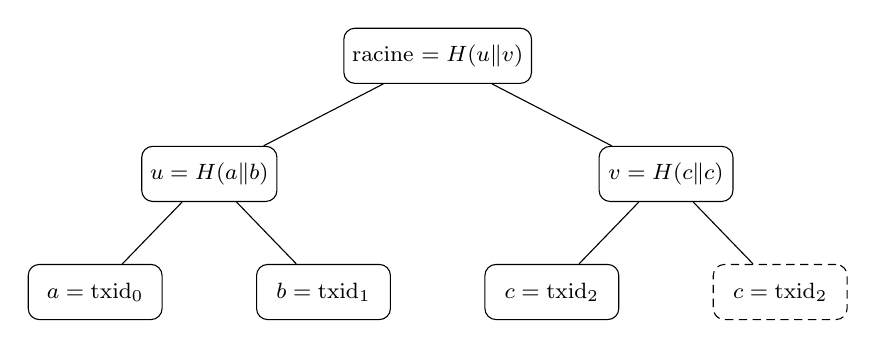
\begin{tikzpicture}[
  level 1/.style={level distance=15mm, sibling distance=58mm},
  level 2/.style={level distance=15mm, sibling distance=29mm},
  every node/.style={draw,rounded corners,inner sep=3pt,font=\footnotesize,minimum width=17mm,minimum height=7mm}]
\node {racine $=H(u\Vert v)$}
  child {node {$u=H(a\Vert b)$}
    child {node {$a=\mathrm{txid}_0$}}
    child {node {$b=\mathrm{txid}_1$}}}
  child {node {$v=H(c\Vert c)$}
    child {node {$c=\mathrm{txid}_2$}}
    child {node[dashed,densely dashed]{$c=\mathrm{txid}_2$}}};
\end{tikzpicture}
\caption{Arbre de Merkle d'un bloc à \textbf{trois} transactions ($\mathrm{txid}_0,\mathrm{txid}_1,
\mathrm{txid}_2$)~: le nombre de feuilles étant impair, le dernier haché $c=\mathrm{txid}_2$ est
\emph{dupliqué} (feuille en pointillés) afin de compléter la paire, puis $v=H(c\Vert c)$.}
\end{figure}

Trois propriétés, énoncées ici sans preuve, structurent la construction et sa vérification.

\begin{proposition}[Terminaison et correction de la construction]\label{prop:correction}
L'algorithme par niveaux \emph{termine}~: la longueur du niveau courant est un entier qui décroît
strictement (variant $\lceil t/2\rceil<t$ dès que $t\ge 2$) jusqu'à valoir $1$. Il est
\emph{correct}~: à chaque étape, chaque n\oe ud est le haché de l'unique couple de ses enfants
(invariant), de sorte que la valeur finale ne dépend que de la liste ordonnée des feuilles.
\end{proposition}

\begin{proposition}[Coût de construction]\label{prop:cout}
Le calcul de la racine de $n$ transactions demande $O(n)$ évaluations de $H$, en temps et espace
$O(n)$, et l'arbre a une hauteur $\lceil\log_2 n\rceil$. La taille d'une preuve d'inclusion, et le
coût de sa vérification, sont donc en $\Theta(\log n)$.
\end{proposition}

\begin{figure}[h]\centering
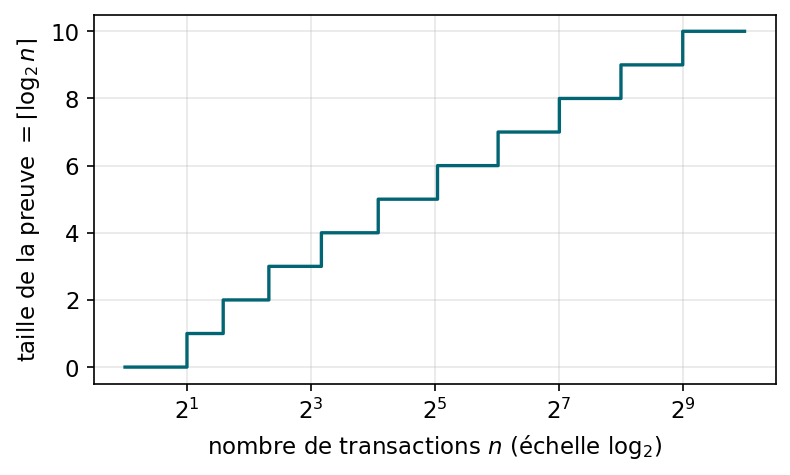
\includegraphics[width=0.6\linewidth]{figs_btc/g1_preuve.png}
\caption{Allure attendue (à obtenir par simulation)~: taille moyenne d'une preuve d'inclusion en
fonction du nombre $n$ de transactions~; on doit retrouver l'escalier $\lceil\log_2 n\rceil$.}
\end{figure}

\begin{remarque}[Une subtilité de sécurité]\label{rem:cve}
La règle de duplication a une conséquence inattendue~: pour certaines valeurs de $n$, un bloc et
un bloc obtenu en dupliquant réellement des transactions peuvent produire la \emph{même} racine
(ambiguïté connue sous le nom de \guillemotleft~CVE-2012-2459~\guillemotright). Une structure
authentifiée doit donc être analysée avec soin~: la racine seule ne garantit pas l'unicité de
l'arbre sous-jacent.
\end{remarque}

\section{Hachage cryptographique et collisions}

La sécurité repose entièrement sur les propriétés de $H$. On distingue la \emph{résistance à la
préimage}, à la \emph{seconde préimage} et aux \emph{collisions}. Cette dernière est cruciale ici.

\begin{proposition}[Existence des collisions]\label{prop:tiroirs}
L'application $H:\{0,1\}^{*}\to\{0,1\}^{256}$ n'est pas injective~: des messages distincts de même
haché existent nécessairement.
\end{proposition}

Les collisions existent donc, mais on \emph{postule} qu'elles sont introuvables en temps
raisonnable (hypothèse \emph{calculatoire}, non un théorème). Sa force se mesure par l'attaque
générique la plus simple, analysée dans le modèle de l'\emph{oracle aléatoire}.

\begin{proposition}[Borne des anniversaires]\label{prop:birthday}
En tirant $k$ valeurs indépendantes et uniformes parmi $M=2^{b}$, la probabilité d'\emph{absence}
de collision vaut $q_k=\prod_{i=0}^{k-1}(1-i/M)$ et vérifie $q_k\le \exp(-k(k-1)/2M)$. Une
collision devient probable dès que $k\gtrsim 1{,}177\cdot 2^{b/2}$.
\end{proposition}

Une empreinte sur $b$ bits n'offre ainsi qu'une résistance de l'ordre de $2^{b/2}$~: le choix
$b=256$ vise une marge de $2^{128}$. Le cas $M=365$ n'est autre que le \emph{paradoxe des
anniversaires}. Ces seuils s'observent par une expérience de Monte-Carlo sur une empreinte
tronquée. La qualité d'une telle estimation est régie par la loi des grands nombres.

\begin{proposition}[Vitesse de convergence de l'estimateur Monte-Carlo]\label{prop:mc}
Un estimateur de Monte-Carlo d'une probabilité (ou d'une espérance) fondé sur $N$ tirages
indépendants a un écart-type en $\Theta(1/\sqrt{N})$~: pour gagner un chiffre décimal de précision,
il faut multiplier $N$ par $100$. En échelle log-log, l'erreur empirique décroît le long d'une
droite de pente $-1/2$.
\end{proposition}

\begin{lstlisting}
import hashlib
def H(m: bytes) -> bytes:
    return hashlib.sha256(hashlib.sha256(m).digest()).digest()
def tronque(h: bytes, b: int) -> int:      # b premiers bits
    return int.from_bytes(h, "big") >> (256 - b)
\end{lstlisting}

\begin{figure}[h]\centering
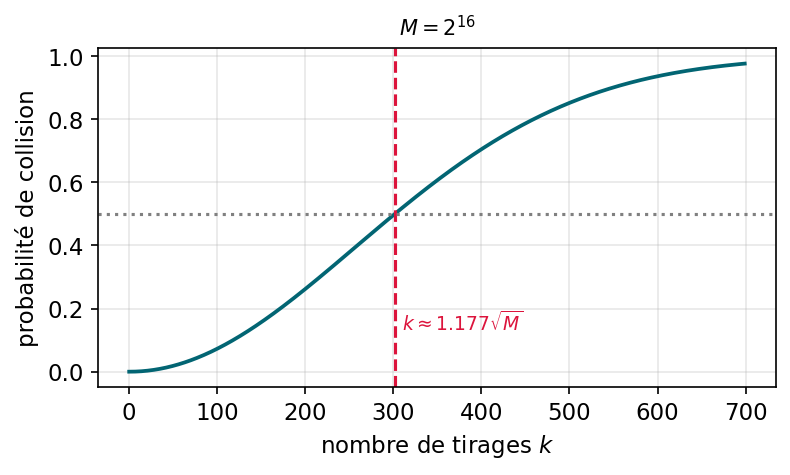
\includegraphics[width=0.58\linewidth]{figs_btc/g2_anniv.png}
\caption{Allure attendue (à obtenir par simulation)~: probabilité d'au moins une collision en
fonction du nombre de tirages, pour une empreinte de $b=16$ bits~; la transition se produit au
voisinage de $1{,}177\sqrt{M}=1{,}177\cdot 2^{8}$.}
\end{figure}

\section{Preuves d'inclusion et clients légers (SPV)}

Un client \emph{léger} (\emph{Simplified Payment Verification}) ne conserve que les en-têtes, donc
les racines. Pour lui prouver qu'une transaction $t$ appartient à un bloc de racine $R$, on lui
fournit une \emph{preuve de Merkle}~: la suite des hachés \emph{frères} rencontrés en remontant de
la feuille $H(t)$ jusqu'à la racine, chacun accompagné de son côté. Le client recombine par $H$ et
accepte si et seulement s'il retrouve $R$. La longueur d'une telle preuve est
$\lceil\log_2 n\rceil=O(\log n)$~: une poignée de hachés là où le bloc entier serait prohibitif.

La sûreté de ce mécanisme se ramène à la seule hypothèse sur $H$.

\begin{theoreme}[Sûreté de la vérification, ou \emph{soundness}]\label{th:soundness}
Si $H$ est résistante aux collisions et si la vérification d'une preuve pour une valeur $x$ aboutit
à la racine authentique $R$, alors --- sauf à exhiber une collision de $H$ --- la valeur $x$
figure réellement parmi les transactions ayant produit $R$.
\end{theoreme}

Autrement dit, forger une fausse preuve d'inclusion \emph{revient à} calculer une collision~: la
sécurité de l'édifice se \emph{réduit} à celle de $H$, ce qui justifie le dimensionnement à $256$
bits. En pratique, un client SPV allège encore ses échanges à l'aide de \emph{filtres de Bloom}
(BIP-37)~: il communique une structure probabiliste identifiant \emph{approximativement} les
transactions qui l'intéressent, acceptant de \guillemotleft~faux positifs~\guillemotright{} pour
préserver un minimum de confidentialité.

\section{Preuve de travail et politique monétaire}

Rester léger suppose de faire confiance à la chaîne d'en-têtes reçue~; Bitcoin la rend coûteuse à
falsifier par la \emph{preuve de travail}. L'en-tête contient un \emph{nonce} $\nu$~; \emph{miner}
le bloc consiste à trouver $\nu$ tel que $H(e_\nu)$, vu comme un entier sur $256$ bits, soit
inférieur à la cible $T$. Dans le modèle de l'oracle aléatoire, chaque essai réussit
indépendamment avec probabilité $p=T/2^{256}$.

\begin{proposition}[Coût du minage]\label{prop:pow}
Le nombre $N$ d'essais jusqu'au premier succès suit une loi géométrique de paramètre $p$~; son
espérance est $\mathbb{E}[N]=1/p$, et le minage termine presque sûrement.
\end{proposition}

Le minage est donc un algorithme \emph{probabiliste} de type Las~Vegas~: résultat toujours
correct, temps aléatoire d'espérance $1/p$. Le protocole \emph{ajuste} périodiquement la cible
--- toutes les $2016$ blocs, soit environ deux semaines --- de manière à maintenir un intervalle
moyen de dix minutes entre blocs, malgré les variations de la puissance de calcul du réseau.

\begin{figure}[h]\centering
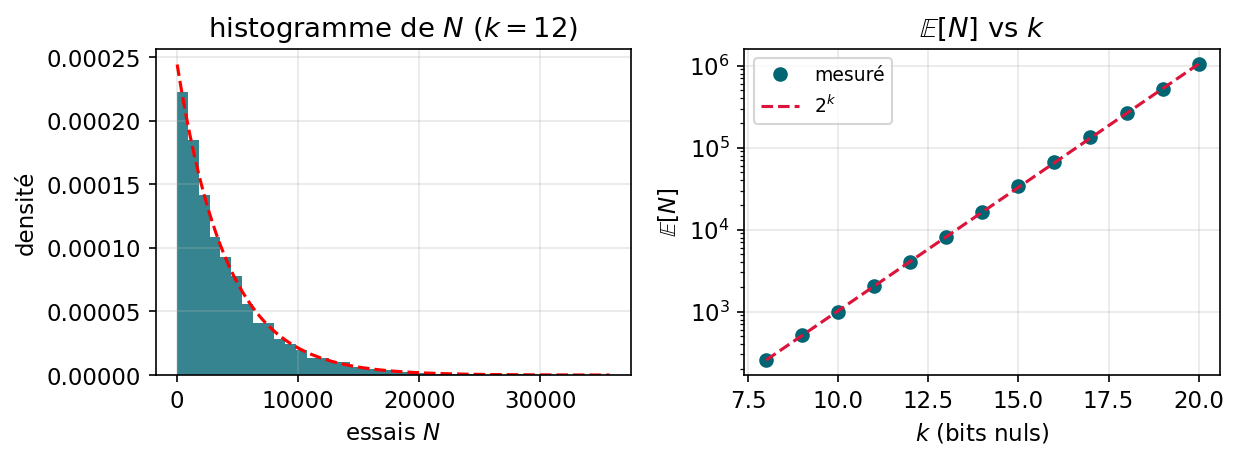
\includegraphics[width=0.92\linewidth]{figs_btc/g3_minage.png}
\caption{Allure attendue (à obtenir par simulation)~: à gauche, l'histogramme du nombre d'essais
$N$ épouse une décroissance géométrique~; à droite, l'espérance mesurée $\mathbb{E}[N]$ suit la
droite $2^{k}$ en échelle semi-logarithmique.}
\end{figure}

La coinbase suit, elle, une \emph{politique monétaire} déterministe~: la subvention par bloc est
divisée par deux tous les $210\,000$ blocs (\emph{halving}). La masse monétaire totale est donc
gouvernée par une série géométrique, dont la convergence est elle-même géométrique.

\begin{proposition}[Masse monétaire bornée et convergence géométrique]\label{prop:supply}
Avec une subvention initiale de $50$~BTC divisée par deux toutes les $210\,000$ blocs, l'émission
totale est majorée par $210\,000\cdot 50\cdot\sum_{i\ge 0} 2^{-i}=21\cdot 10^{6}$~BTC. De plus,
après la $e$-ième ère de halving, la fraction déjà émise vaut $1-2^{-(e+1)}$~: l'écart au plafond
décroît \emph{géométriquement} en $2^{-e}$.
\end{proposition}

\begin{figure}[h]\centering
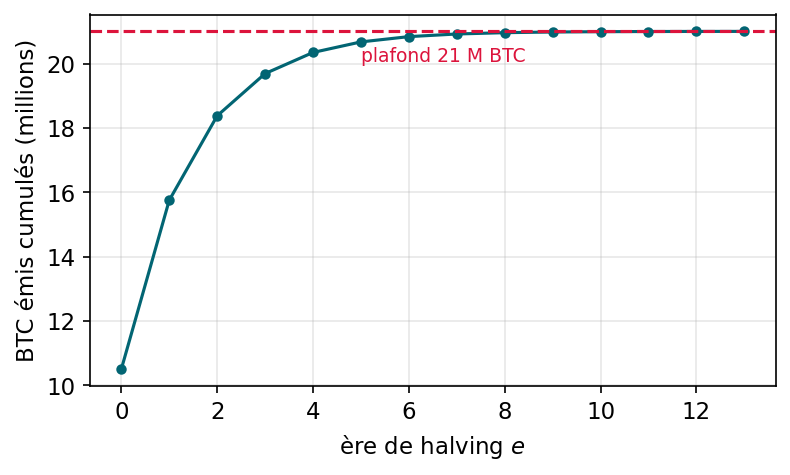
\includegraphics[width=0.58\linewidth]{figs_btc/g4_supply.png}
\caption{Allure attendue (à obtenir par simulation)~: BTC cumulés émis au fil des ères de halving,
convergeant géométriquement vers le plafond de $21$~millions.}
\end{figure}

Enfin, la \emph{sécurité} de la chaîne se lit comme une course~: un attaquant de puissance
relative $\alpha<1/2$, parti avec $z$ blocs de retard, ne rattrape la chaîne honnête qu'avec une
probabilité décroissant exponentiellement en $z$. C'est le fondement de la règle des
\emph{confirmations} et le lien entre la vérification légère du client et la robustesse du
consensus.

\section{Structures voisines}

L'arbre binaire de Bitcoin admet des variantes. Ethereum emploie un arbre de \emph{Patricia-Merkle}
pour indexer un état modifiable~; les \emph{arbres de Verkle} remplacent le hachage par des
\emph{engagements polynomiaux} et abaissent la taille des preuves de $O(\log n)$ à $O(1)$. Plus
généralement, la vérification \guillemotleft~à faible coût~\guillemotright{} illustrée ici inspire
les \emph{preuves à divulgation nulle} et les \emph{rollups}.

\section*{Suggestions pour le développement}

\emph{Pistes largement indépendantes~; on n'en traitera qu'une partie, en privilégiant celles que
l'on peut à la fois exposer, implémenter et éprouver par une simulation.}

\begin{itemize}[nosep,leftmargin=1.3em]
  \item Prouver la Proposition~\ref{prop:correction} (terminaison via le variant, correction via
        l'invariant) puis la Proposition~\ref{prop:cout}~; implémenter la construction, la
        génération et la vérification des preuves, et retrouver expérimentalement l'escalier
        $\lceil\log_2 n\rceil$ (Figure~2).
  \item Démontrer la Proposition~\ref{prop:birthday}, en discuter l'équivalent asymptotique et la
        confronter à une expérience de Monte-Carlo (Figure~3)~; établir la
        Proposition~\ref{prop:mc} et vérifier la pente $-1/2$ en échelle log-log.
  \item Prouver le Théorème~\ref{th:soundness} et expliciter la \emph{réduction}~: comment une
        fausse preuve fournit-elle effectivement une collision~?
  \item Approfondir la Remarque~\ref{rem:cve}~: caractériser les tailles de blocs sensibles à
        l'ambiguïté de duplication et proposer une parade.
  \item Étudier et simuler le modèle de minage (Proposition~\ref{prop:pow})~: distribution de $N$,
        effet de l'ajustement de difficulté, temps moyen entre blocs.
  \item Établir la Proposition~\ref{prop:supply}, mettre en évidence la convergence géométrique
        vers $21$~millions (Figure~5) et discuter la place des frais lorsque la subvention s'éteint.
  \item Modéliser et simuler la \guillemotleft~course entre chaînes~\guillemotright{}~: probabilité
        de rattrapage en fonction de $\alpha$ et $z$~; en déduire un choix du nombre de confirmations.
  \item Analyser les filtres de Bloom (BIP-37)~: taux de faux positifs, compromis
        confidentialité/bande passante pour un client SPV.
  \item Comparer, en complexité et en taille de preuve, l'arbre binaire de Bitcoin, un arbre
        $k$-aire, l'arbre de Patricia-Merkle et les engagements de type Verkle.
\end{itemize}

\section*{Références}
\begin{enumerate}[nosep,leftmargin=1.6em]
  \item S.~Nakamoto, \emph{Bitcoin: A Peer-to-Peer Electronic Cash System}, 2008.
  \item R.~C.~Merkle, \emph{A digital signature based on a conventional encryption function}, CRYPTO~'87.
  \item A.~M.~Antonopoulos, \emph{Mastering Bitcoin}, O'Reilly~; A.~M.~Antonopoulos, G.~Wood,
        \emph{Mastering Ethereum}, O'Reilly.
  \item J.~Katz, Y.~Lindell, \emph{Introduction to Modern Cryptography}, CRC Press.
\end{enumerate}

\vfill
\noindent\rule{\linewidth}{0.3pt}\\
{\footnotesize\itshape Texte de modélisation proposé dans le cadre d'une préparation à
l'agrégation d'informatique par Pr Agrégé El Hadiq Zouhair --- \href{https://cpgeacademy.org}{cpgeacademy.org}.}

\end{document}
